\documentclass[a4paper,12pt]{article}
\usepackage[a4paper, total={6in, 8in}]{geometry}
\usepackage[spanish]{babel}
\usepackage[utf8]{inputenc}
\usepackage{cite}
\usepackage{graphicx}
\usepackage{flushend}
% Paquetes de la AMS:
\usepackage{amsmath, amsthm, amsfonts}
\usepackage{hyperref}
\usepackage{textcomp}

% Teoremas
%--------------------------------------------------------------------------
\newtheorem{thm}{Teorema}[section]
\newtheorem{cor}[thm]{Corolario}
\newtheorem{lem}[thm]{Lema}
\newtheorem{prop}[thm]{Proposici?n}
\theoremstyle{definition}
\newtheorem{defn}[thm]{Definici?n}
\theoremstyle{remark}
\newtheorem{rem}[thm]{Observaci?n}
\newcommand\blankpage{%
    \null
    \thispagestyle{empty}%
    \addtocounter{page}{0}%
    \newpage}
% Atajos.
% Se pueden definir comandos nuevos para acortar cosas que se usan
% frecuentemente. Como ejemplo, aqu? se definen la R y la Z dobles que
% suelen representar a los conjuntos de n?meros reales y enteros.
%--------------------------------------------------------------------------

\def\RR{\mathbb{R}}
\def\ZZ{\mathbb{Z}}

% De la misma forma se pueden definir comandos con argumentos. Por
% ejemplo, aqu? definimos un comando para escribir el valor absoluto
% de algo m?s f?cilmente.
%--------------------------------------------------------------------------
\newcommand{\abs}[1]{\left\vert#1\right\vert}

% Operadores.
% Los operadores nuevos deben definirse como tales para que aparezcan
% correctamente. Como ejemplo definimos en jacobiano:
%--------------------------------------------------------------------------
\DeclareMathOperator{\Jac}{Jac}

%--------------------------------------------------------------------------
\usepackage{minted}
\begin{document}
\begin{titlepage}
	\centering
	\begin{figure}[h]
    \centering
    
\includegraphics[width=0.3\textwidth]{figures/log_uni.png}
    \end{figure}
    
	{\scshape\huge Universidad Nacional de Ingeniería\par
	\Large Facultad de Ciencias\par
	\large Maestría en Ciencias de la Computación\par}
	\vspace{1cm}
	{\LARGE \itshape Análisis de Sentimientos en Tiempo Real de Tweets usando SVM y Aprendizaje Supervisado\par}
	\vspace{1cm}
	{\scshape\large\textbf{Informe Final}\par}
	{\scshape\large Procesamiento de Lenguaje Natural\par}

    \vspace{.5cm}
	{\large\itshape 
	Joel Hancco\par
	Franz Maguiña\par
	Eduardo Rashta\par
	Jhon Vargas\par\vspace{.5cm}
	Profesor: Erasmo Gómez\par}
    \vspace{.5cm}
    % Bottom of the page
	{\large \today\par}
\end{titlepage}

\begin{abstract}
\end{abstract}

\newpage
\tableofcontents
\newpage
\section{Introducción}

En el presente informe se detalla una solución sobre el análisis de sentimientos de Tweets recopilados a través de la API de Twitter, también se detalla sobre el tratamiento de los Tweets. Y mediante una aplicación web hecha en Flask, se interactúa con el modelo extrayendo, visualizando y analizando Tweets en tiempo real.

\section{Objetivos}

El objetivo general del proyecto es la aplicación de métodos de Machine Learning como métodos de SVM y de Aprendizaje Supervisado sobre Tweets para determinar las características de los sentimientos de los mismos en tiempo real.\\

Mientras que los objetivos secundarios son:

\begin{itemize}
    \item Determinar que métodos de extracción de Tweets son más eficientes, a través de Web Scrapping o API.
    \item Determinar que modelo es de mayor utilidad, clasificación SVM o métodos de Aprendizaje Supervisado.
    \item Desarrollar una interfaz web que permita la interacción de un usuario con el modelo.
\end{itemize}

\section{Estado del Arte}
\subsection{Métodos de Extracción de Tweets}
\subsubsection{Web Scrapping}
Web scrapping, web harvesting o web data extraction consiste en la extracción de datos de páginas web mediante librerias que tienen acceso a World Wide Web utilizan el protocolo de transferencia de hipertexto. Si bien este proceso puede ser replicado por una persona y un navegador web.\\

Los métodos de Web Scrapping son métodos automatizados, que básicamente busca en la sintaxis de la pagina web, datos de importancia que están en un lugar en especifico de la web, entre etiquetas de HTML generalmente. Esta recopilación se guarda en una variable, archivo o base de datos para su posterior tratamiento y análisis.


\begin{figure}[htb]
\centering
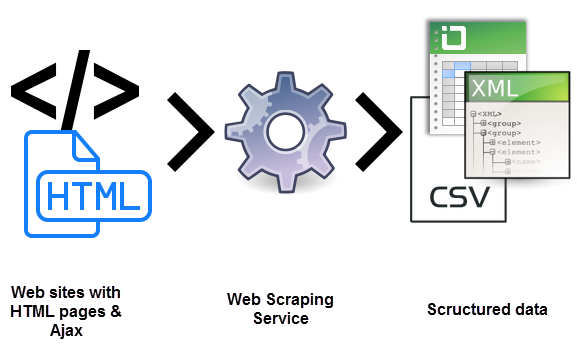
\includegraphics[width=0.75\textwidth]{figures/web-scraping-service.png}
\caption{Proceso de Web Scrapping}
%\label{fig:f3}
\end{figure}

\subsubsection{API de Twitter}
La API (Application Programming Interface) de Twitter provee las herramientas para contribuir, interactuar y analizar la conversación que sucede en Twitter. Usado frecuentemente para recuperar y analizar datos mediante programación, asi como para participar en la conversación en Twitter. El listado de recursos que proporciona la API de Twitter es la siguiente:
\begin{itemize}
    \item Tweets
    \item Usuarios
    \item Mensajes Directos
    \item Listas
    \item Imágenes y Videos
    \item Lugares
\end{itemize}

Para tener accesos a esta herramienta es necesario registrarse en Twitter y usar las opciones para programadores, generando las credenciales de acceso a la API de Twitter.

\begin{figure}[htb]
\centering

\includegraphics[width=0.75\textwidth]{figures/twitter-api.jpg}
\caption{Logo de la API de Twitter}
%\label{fig:f3}
\end{figure}

\subsection{Métodos de Machine Learning}

\subsubsection{SVM}


\subsubsection{Aprendizaje Supervisado}



\subsection{Investigaciones Previas}
\subsubsection{Sentiment analysis in tweets: an assessment study from classical tomodern text representation models}

\subsubsection{Practical Text Classification With Large Pre-Trained Language Models}

\subsubsection{XLM-T:A Multilingual Language Model Toolkit for Twitter}

\subsubsection{Using millions of emoji occurrences to learn any-domain representationsfor detecting sentiment, emotion and sarcasm}

\subsection{Framework Flask}
\textbf{Flask} es un micro framework web escrito Python que permite crear aplicaciones web rápidamente y con un mínimo número de líneas de código. Clasificado como micro framework porque no requiere otras herramientas o bibliotecas particulares.\\

Además, Flask no tiene una capa de abstracción de base de datos, validación de formularios ni ningún otro componente donde las bibliotecas de terceros preexistentes proporcionan funciones comunes. Sin embargo, Flask admite extensiones que pueden agregar funciones de la aplicación como si estuvieran implementadas en el propio Flask. Existen extensiones para mapeadores relacionales de objetos, validación de formularios, manejo de carga, varias tecnologías de autenticación abierta y varias herramientas comunes relacionadas con el framework.\\

Aplicaciones que usan Flask como framework son Pinterest y LinkedIn

\begin{figure}[htb]
\centering

\includegraphics[width=0.5\textwidth]{figures/1024px-Flask_logo.png}
\caption{Logo de Flask}
%\label{fig:f3}
\end{figure}





\section{Metodología}
\subsection{Extracción de Datos}

Para extraer los datos, se utilizó las técnicas de Web Scrapping y la conexión a la API de Twitter:
\subsubsection{Web Scrapping}

Antes de aplicar los métodos de Web Scrapping, es necesario realizar algunas configuraciones, como la autentificación en el sitio web.\\

\textbf{Librerias a usar}

\begin{minted}
[
frame=lines,
framesep=2mm,
baselinestretch=1.2,
fontsize=\footnotesize,
linenos
]{python}
import csv
from getpass import getpass
from time import sleep
import pandas as pd
from selenium.webdriver.common.keys import Keys
from selenium.common.exceptions import NoSuchElementException
from selenium import webdriver
chrome_options = webdriver.ChromeOptions()
chrome_options.add_argument('--start-maximized')
#chrome_options.add_argument('--incognito')
chrome_options.add_argument('--headless')
driver =webdriver.Chrome('chromedriver', options=chrome_options)
 \end{minted}

\textbf{Autentificación}\\

Mediante el siguiente código se realiza la autentificación a una cuenta de Twitter.

\begin{minted}
[
frame=lines,
framesep=2mm,
baselinestretch=1.2,
fontsize=\footnotesize,
linenos
]{python}
driver.get('https://www.twitter.com/login')
sleep(1)
username = driver.find_element_by_xpath('//input[@name="session[username_or_email]"]')
username.send_keys('your_keys')
#pln_user
password = 'pln_user'
my_password = getpass(password)
password = driver.find_element_by_xpath('//input[@name="session[password]"]')
password.send_keys(my_password)

password.send_keys(Keys.RETURN)
sleep(1)
\end{minted}


\textbf{Tendencias para Perú}\\

Mediante el siguiente código se realiza la obtención de temas o tópicos que están siendo tendencia en cierta región como Perú por ejemplo.

\begin{minted}
[
frame=lines,
framesep=2mm,
baselinestretch=1.2,
fontsize=\footnotesize,
linenos
]{python}
driver.find_element_by_xpath('//a[@href="/explore"]').click()
sleep(2)
list_trends = driver.find_elements_by_xpath('//div[@data-testid="trend"]')
list_trend = []
for trend in list_trends:
    if trend.find_element_by_xpath('.//div[1]/div[1]').text == "Trending in Peru":
        list_trend.append(trend.find_element_by_xpath('.//div[1]/div[2]').text)

list_trend
\end{minted}

Teniendo como resultado las tendencias mostradas en la figura \ref{fig:ws_trends}

\begin{figure}[htb]
\centering
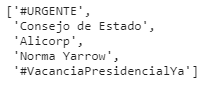
\includegraphics{figures/trends.png}
\caption{Tendencias en Perú}
\label{fig:ws_trends}
\end{figure}

\textbf{Función \textit{get\_tweet\_data}}\\

Mediante la siguiente función se realiza el método de Web Scrapping.

\begin{minted}
[
frame=lines,
framesep=2mm,
baselinestretch=1.2,
fontsize=\footnotesize,
linenos
]{python}
def get_tweet_data(card):
    """Extract data from tweet card"""
    username = card.find_element_by_xpath(".//span").text
    try:
        handle = card.find_element_by_xpath('.//span[contains(text(), "@")]').text
    except NoSuchElementException:
        return
    try:
        postdate = card.find_element_by_xpath(".//time").get_attribute("datetime")
    except NoSuchElementException:
        return
    comment = card.find_element_by_xpath(".//div[2]/div[2]/div[1]").text
    responding = card.find_element_by_xpath(".//div[2]/div[2]/div[2]").text
    text = comment + responding
    reply_cnt = card.find_element_by_xpath('.//div[@data-testid="reply"]').text
    retweet_cnt = card.find_element_by_xpath('.//div[@data-testid="retweet"]').text
    like_cnt = card.find_element_by_xpath('.//div[@data-testid="like"]').text

    # get a string of all emojis contained in the tweet
    """Emojis are stored as images... so I convert the filename,
    which is stored as unicode, into the emoji character."""
    emoji_tags = card.find_elements_by_xpath('.//img[contains(@src, "emoji")]')
    emoji_list = []
    for tag in emoji_tags:
        filename = tag.get_attribute("src")
        try:
            emoji = chr(
                int(re.search(r"svg\/([a-z0-9]+)\.svg", filename).group(1), base=16)
            )
        except AttributeError:
            continue
        if emoji:
            emoji_list.append(emoji)
    emojis = " ".join(emoji_list)

    tweet = (username, handle, postdate, text, emojis, reply_cnt, retweet_cnt, like_cnt)
    return tweet
\end{minted}

\textbf{Extracción de Tweets}\\

Mediante la siguiente función se realiza el método de extracción de Tweets de los temas en tendencia extraído anteriormente.

\begin{minted}
[
frame=lines,
framesep=2mm,
baselinestretch=1.2,
fontsize=\footnotesize,
linenos
]{python}
df = pd.DataFrame(columns = ['Trend','UserName', 'Handle', 'Timestamp',
                             'Text', 'Emojis', 'Comments', 'Likes', 'Retweets'])
for trend in list_trend:
    
    search_term = trend + " Perú"
    search_input = driver.find_element_by_xpath('//input[@aria-label="Search query"]')
    search_input.send_keys(Keys.CONTROL + 'a')
    search_input.send_keys(Keys.BACK_SPACE)
    search_input.send_keys(search_term)
    search_input.send_keys(Keys.RETURN)
    sleep(6)

    driver.find_element_by_link_text('Latest').click()
    
    import re
    
    data = []
    tweet_ids = set()
    last_position = driver.execute_script("return window.pageYOffset;")
    scrolling = True

    for i in range(0,9):
        page_cards = driver.find_elements_by_xpath('//div[@data-testid="tweet"]')
        for card in page_cards[-15:]:
            tweet = get_tweet_data(card)
            #print(tweet)
            if tweet:
                tweet_id = ''.join(tweet)
                if tweet_id not in tweet_ids:
                    tweet_ids.add(tweet_id)
                    payload = [trend] + list(tweet)
                    #print(payload)
                    series_obj = pd.Series(payload,index = df.columns)
                    df = df.append(series_obj,ignore_index = True)

        scroll_attempt = 0
        temp = True
        while temp:
            # check scroll position
            driver.execute_script('window.scrollTo(0, document.body.scrollHeight);')
            sleep(2)
            curr_position = driver.execute_script("return window.pageYOffset;")
            if last_position == curr_position:
                scroll_attempt += 1

                # end of scroll region
                if scroll_attempt >= 3:
                    scrolling = False
                    temp = False
                    break
                else:
                    sleep(2) # attempt another scroll
            else:
                last_position = curr_position
                break
                
# close the web driver
driver.close()
\end{minted}

Teniendo como resultado el DataFrame mostrado en la figura \ref{fig:ws_df}

\begin{figure}[htb]
\centering
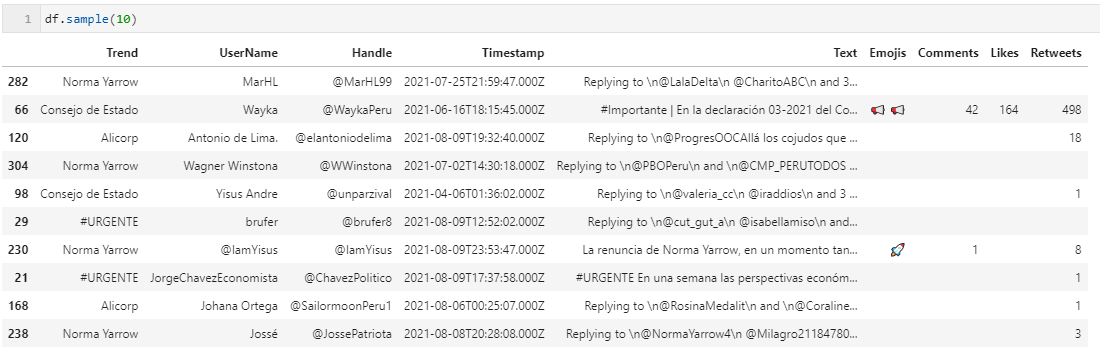
\includegraphics[width=\textwidth]{figures/df_ws.png}
\caption{Tendencias en Perú}
\label{fig:ws_df}
\end{figure}

\subsubsection{API de Twitter}

Antes de utilizar la API de Twitter es realiza los siguientes pasos.\\

\textbf{Librerías a usar}


\begin{minted}
[
frame=lines,
framesep=2mm,
baselinestretch=1.2,
fontsize=\footnotesize,
linenos
]{python}
import os
import tweepy as tw
import numpy as np
import pandas as pd
import json 
\end{minted}

\textbf{Configuración de variables con los Tokens}\\

Mediante el siguiente código se configura los tokens generados en la cuenta de la API de Twitter. 


\begin{minted}
[
frame=lines,
framesep=2mm,
baselinestretch=1.2,
fontsize=\footnotesize,
linenos
]{python}
consumer_key = 'consumer_key'
consumer_secret = 'consumer_secret'
access_token = 'access_token'
access_token_secret = 'access_token_secret'

auth = tw.OAuthHandler(consumer_key, consumer_secret)
auth.set_access_token(access_token, access_token_secret)
api = tw.API(auth, wait_on_rate_limit=True, wait_on_rate_limit_notify=True)

\end{minted}


\textbf{Función para acceder por fecha a Tweets}\\

La siguiente función muestra la obtención de Tweets por fechas usando la API de Twitter.

\begin{minted}
[
frame=lines,
framesep=2mm,
baselinestretch=1.2,
fontsize=\footnotesize,
linenos
]{python}
def tweet_days(search_words, month, day):

    dt = datetime.datetime.today()
    year = dt.year
    date_since = datetime.datetime(year, month, day, 0, 0, 0)
    date_until =   datetime.datetime(year, month, day+1, 0, 0, 0)

    tweets = tw.Cursor(api.search,
                       q=search_words,
                       lang="en",
                       since=date_since,
                       until=date_until,
                       result_type="recent",
                       sleep_on_rate_limit=False
                       ).items(25)

    return tweets
\end{minted}



\textbf{Función para recopilar Tweets en DataFrame}

\begin{minted}
[
frame=lines,
framesep=2mm,
baselinestretch=1.2,
fontsize=\footnotesize,
linenos
]{python}
def get_tweets(search_words):

    df = pd.DataFrame(columns=['date', 'user', 'text'])

    date_since = datetime.datetime(2021, 7, 1, 0, 0, 0)
    #date_until =   datetime.datetime(year, month, day+1, 0, 0, 0)

    tweets = tw.Cursor(api.search,
                       q=search_words,
                       lang="en",
                       since=date_since,
                       #until=date_until,
                       result_type="recent",
                       sleep_on_rate_limit=False
                       ).items(1000)
    data = [[tweet.created_at, tweet.user.screen_name, tweet.text] for tweet in tweets]
    df = pd.DataFrame(data = data, columns=['date', 'user', 'text'])
    return df
\end{minted}







\subsection{Tratamiento de Datos}

El proceso de tratamiento de datos, consiste en normalizar el texto extraido, quitar caracteres especiales, remover espacios demás, cambiar vocales con tildes a que estén sin tilde y también, quitar los signos de puntuación.\\

Para lograr esto, se realiza el siguiente procedimiento.\\

\textbf{Librerías a Usar}

\begin{minted}
[
frame=lines,
framesep=2mm,
baselinestretch=1.2,
fontsize=\footnotesize,
linenos
]{python}
import nltk
nltk.download('punkt')
nltk.download('stopwords')
nltk.download('wordnet')

from nltk import word_tokenize
from nltk.corpus import stopwords
from nltk.stem import PorterStemmer, WordNetLemmatizer, SnowballStemmer
from nltk import FreqDist
import re
\end{minted}



\textbf{Proceso a los datos extraídos por Web Scrapping}\\

Para los datos extraidos por Web Scrapping se realiza la limpieza de texto de la siguiente forma:

\begin{minted}
[
frame=lines,
framesep=2mm,
baselinestretch=1.2,
fontsize=\footnotesize,
linenos
]{python}
stopwords = stopwords.words('spanish')
def text_prep(text:str):
    tokens = [] 
    text = re.sub('https\S+', '', text)
    text = re.sub('Replying to \n@\S+', '', text)
    text = re.sub('and \n@\S+', '', text)
    text = re.sub('\n@\S+', '', text)
    text = re.sub('#\S+', '', text)
    
    text = text.replace('á','a').replace('é','e')\
               .replace('í','i').replace('ó','o')\
               .replace('ú','u')
    for w in word_tokenize(text):
        w = w.lower()
        if ((re.search('[a-zA-Z]', w)) and (w not in stopwords)): tokens.append(w)
    return ' '.join(tokens)
\end{minted}

Obteniéndose una nueva columna al DataFrame de los datos extraidos por Web Scrapping mostrado en la figura \ref{fig:ws_tf}

\begin{figure}[htb]
\centering
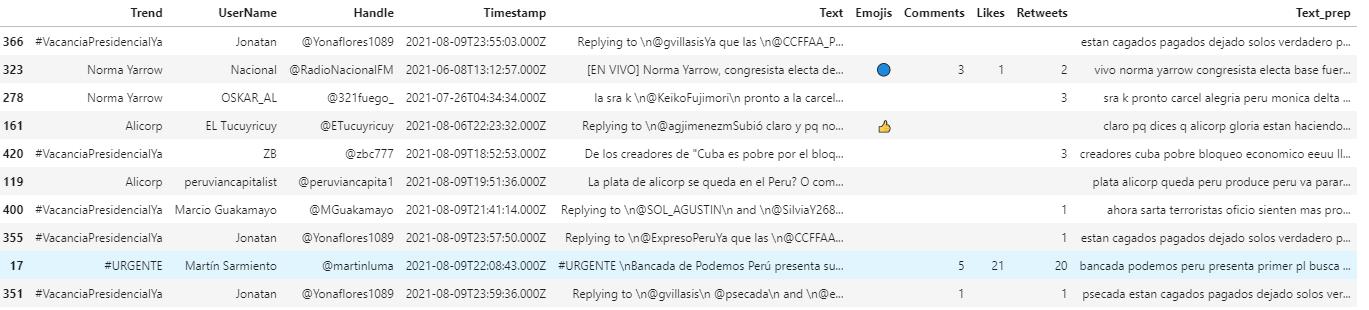
\includegraphics[width=\textwidth]{figures/df_tf.png}
\caption{Dataframe con la columna de texto preprocesado}
\label{fig:ws_tf}
\end{figure}

\textbf{Proceso a los datos extraídos por la API de Twitter}\\

Para los datos extraidos mediante la API de Twitter  se realiza la limpieza de texto de la siguiente forma:


\begin{minted}
[
frame=lines,
framesep=2mm,
baselinestretch=1.2,
fontsize=\footnotesize,
linenos
]{python}
def text_prep(text:str):
    from nltk.corpus import stopwords
    stopwords = stopwords.words('english')
    
    tokens = [] 
    text = re.sub('https\S+', '', text)
    regrex_pattern = re.compile(pattern = "["
        u"\U0001F600-\U0001F64F"  # emoticons
        u"\U0001F300-\U0001F5FF"  # symbols & pictographs
        u"\U0001F680-\U0001F6FF"  # transport & map symbols
        u"\U0001F1E0-\U0001F1FF"  # flags (iOS)
        u"\U00002500-\U00002BEF"  # chinese char
        u"\U00002702-\U000027B0"
        u"\U00002702-\U000027B0"
        u"\U000024C2-\U0001F251"
        u"\U0001f926-\U0001f937"
        u"\U00010000-\U0010ffff"
        u"\u2640-\u2642" 
        u"\u2600-\u2B55"
        u"\u200d"
        u"\u23cf"
        u"\u23e9"
        u"\u231a"
        u"\ufe0f"  # dingbats
        u"\u3030"
        "]+", flags = re.UNICODE)

    text = regrex_pattern.sub(r'',text)
    #text = re.sub('Replying to \n@\S+', '', text)
    text = re.sub('RT @\S+', '', text)
    text = re.sub('@\S+', '', text)
    text = re.sub('#\S+', '', text)

    for w in word_tokenize(text):
        w = w.lower()
        if ((re.search('[a-zA-Z]', w)) and (w not in stopwords)): tokens.append(w)
    return ' '.join(tokens)
\end{minted}

\textbf{}

\begin{minted}
[
frame=lines,
framesep=2mm,
baselinestretch=1.2,
fontsize=\footnotesize,
linenos
]{python}

\end{minted}

\textbf{}

\begin{minted}
[
frame=lines,
framesep=2mm,
baselinestretch=1.2,
fontsize=\footnotesize,
linenos
]{python}

\end{minted}

\textbf{}

\begin{minted}
[
frame=lines,
framesep=2mm,
baselinestretch=1.2,
fontsize=\footnotesize,
linenos
]{python}

\end{minted}


\subsection{Extracción de Patrones y Descripción de Insights}



\subsection{Arquitectura de los Modelos}



\section{Experimentación y Resultados}

\section{Recomendación y Trabajo Futuro}

\section{Conclusión y Trabajos Futuros}

\begin{thebibliography}{00}
\bibitem{b1} Sergio Barreto, Ricardo Moura, Jonnathan Carvalho, Aline Paes, Alexandre Plastino (2021) Sentiment analysis in tweets: an assessment study from classical to modern text representation models. Enlace Paper: \href{https://arxiv.org/pdf/2105.14373v1.pdf}{https://arxiv.org/pdf/2105.14373v1.pdf}.

\bibitem{b2} Neel Kan, Raul Puri, Nikolai Yakovenko, Bryan Catanzaro (2018) Practical Text Classification With Large Pre-Trained Language Models. Enlace Paper: \href{https://arxiv.org/pdf/1812.01207v1.pdf}{https://arxiv.org/pdf/1812.01207v1.pdf}.

\bibitem{b3} Francesco Barbieri, Luis Espinosa Anke,  Jose Camacho-Collados (2021) XLM-T: A Multilingual Language Model Toolkit for Twitter. Enlace Paper: \href{https://arxiv.org/pdf/2104.12250v1.pdf}{https://arxiv.org/pdf/2104.12250v1.pdf}.

\bibitem{b4} Bjarke Felbo, Alan Mislove,  Anders Søgaard, Iyad Rahwan, Sune Lehmann (2017) Using millions of emoji occurrences to learn any-domain representations for detecting sentiment, emotion and sarcasm. Enlace Paper: \href{https://arxiv.org/pdf/1708.00524v2.pdf}{https://arxiv.org/pdf/1708.00524v2.pdf}.

\bibitem{b5} Documentación Oficial de Flask. Enlace: \href{https://flask.palletsprojects.com/en/2.0.x/}{https://flask.palletsprojects.com/en/2.0.x/}

\bibitem{b6} Documentación Oficial de Twitter. Enlace: \href{https://developer.twitter.com/en/docs/twitter-api}{https://developer.twitter.com/en/docs/twitter-api}

\end{thebibliography}

\end{document}












